% ============================================================
% Appendix B — Additional Analyses
% ============================================================

\section{Additional Analyses}
\label{sec:appendix_additional}

\subsection{Contaminated-Training (No-Excision) Condition Results}
\label{sec:contaminated_results}

The anomaly-excised condition of the main comparison grants each unsupervised baseline the most
favorable pre-processing benefit from the available labels: excision of contaminated training
regions.
Table~\ref{tab:contaminated} reports the complementary contaminated-training condition, in which
the same 22 unsupervised baselines train on the full contaminated stream without excision,
quantifying the performance penalty of unaddressed contamination for each method family and
contextualizing the training-volume asymmetry acknowledged in Section~\ref{sec:baselines}.

% ---- Table B.1 placeholder ----
\begin{table*}[tp]
\footnotesize
\centering
\caption{Contaminated-training (no-excision) condition results for all 22 unsupervised
  baselines. Each method trains on the identical contaminated training stream used by CSMAD
  (no anomaly excision; labels unused) and is evaluated on the identical held-out evaluation
  half. Metrics: PA\%K-AUC F1 and VUS-PR per dataset family; $\Delta$ columns give the change
  relative to the anomaly-excised condition of Table~\ref{tab:main_results} (positive =
  contaminated-training better). The CSMAD row is repeated from Table~\ref{tab:main_results}
  for reference, as CSMAD trains on the contaminated stream in both conditions.}
\label{tab:contaminated}
\begin{adjustbox}{max width=\linewidth}
\begin{tabular}{lcccccc}
\toprule
& \multicolumn{2}{c}{SWaT excl22} & \multicolumn{2}{c}{PSM} & \multicolumn{2}{c}{SMD avg} \\
\cmidrule(lr){2-3}\cmidrule(lr){4-5}\cmidrule(lr){6-7}
Method & F1 & $\Delta$ & F1 & $\Delta$ & F1 & $\Delta$ \\
\midrule
CSMAD (reference) & {[X.XX]} & --- & {[X.XX]} & --- & {[X.XX]} & --- \\
\multicolumn{7}{c}{\textit{(22 unsupervised baseline rows; cells pending)}} \\
\bottomrule
\end{tabular}
\end{adjustbox}
\end{table*}

\subsection{Epoch-Budget Sensitivity}
\label{sec:epoch_sensitivity}

Section~\ref{sec:impl} reported the asymmetric training budgets (500\,/\,50\,/\,10 epochs).
To assess whether this asymmetry materially affects the comparison, representative unsupervised
baselines are re-trained at extended budgets, and CSMAD is re-trained at a reduced budget, under
the otherwise unchanged protocol.

% ---- Table B.2 placeholder ----
\begin{table*}[tp]
\footnotesize
\centering
\caption{Epoch-budget sensitivity. PA\%K-AUC F1 of representative unsupervised baselines
  trained for 10 (main budget), 50, and 100 epochs, and of CSMAD trained for 500 (main budget)
  and a reduced budget, on representative datasets; best-epoch selection identical to the main
  protocol (Section~\ref{sec:impl}).}
\label{tab:epoch_sensitivity}
\begin{adjustbox}{max width=\linewidth}
\begin{tabular}{lcccc}
\toprule
Method & 10 epochs & 50 epochs & 100 epochs & 500 epochs \\
\midrule
Anomaly Trans. & {[X.XX]} & {[X.XX]} & {[X.XX]} & --- \\
TranAD         & {[X.XX]} & {[X.XX]} & {[X.XX]} & --- \\
CSMAD          & --- & --- & {[X.XX]} & {[X.XX]} \\
\bottomrule
\end{tabular}
\end{adjustbox}
\end{table*}

\subsection{Computational Cost}
\label{sec:cost}

Leave-one-out inference (Section~\ref{sec:scoring}) performs approximately $N=50$ forward passes
per window.
Table~\ref{tab:compute} reports measured per-window FLOPs, end-to-end wall-clock evaluation
time, and peak GPU memory against single-mask scoring; the measured wall-clock overhead factor
is [X.XX].
% PH:NUM-031 | measured wall-clock overhead factor

% ---- Table B.3 placeholder ----
\begin{table*}[tp]
\footnotesize
\centering
\caption{Computational cost of CSMAD inference: per-window forward FLOPs, end-to-end wall-clock
  evaluation time, and peak GPU memory for leave-one-out masking versus single-mask scoring,
  measured on representative datasets (hardware of \ref{sec:appendix_impl}).}
\label{tab:compute}
\begin{adjustbox}{max width=\linewidth}
\begin{tabular}{lccc}
\toprule
Scoring mode & FLOPs / window & Wall-clock (s/entity) & Peak GPU mem.\ (GB) \\
\midrule
Single-mask   & {[X.XX]} & {[X.XX]} & {[X.XX]} \\
Leave-one-out & {[X.XX]} & {[X.XX]} & {[X.XX]} \\
Overhead $\times$ & {[X.XX]} & {[X.XX]} & --- \\
\bottomrule
\end{tabular}
\end{adjustbox}
\end{table*}

\subsection{Parameter Sensitivity}
\label{sec:param_sensitivity}

% ---- Figure B.1 placeholder ----
\begin{figure}[h]
  \centering
  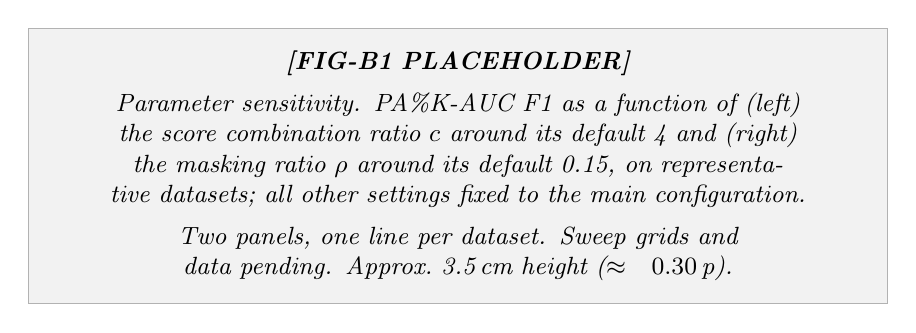
\begin{tikzpicture}
    \node[draw=gray!60, fill=gray!10, minimum width=0.90\linewidth, minimum height=3.5cm,
          text width=0.86\linewidth, align=center, font=\small\itshape] (box) {%
      \textbf{[FIG-B1 PLACEHOLDER]}\\[4pt]
      Parameter sensitivity. PA\%K-AUC F1 as a function of
      (\textit{left}) the score combination ratio $c$ around its default 4 and
      (\textit{right}) the masking ratio $\rho$ around its default 0.15,
      on representative datasets; all other settings fixed to the main configuration.\\[4pt]
      Two panels, one line per dataset. Sweep grids and data pending.
      Approx.\ 3.5\,cm height ($\approx 0.30$\,p).
    };
  \end{tikzpicture}
  \caption{Parameter sensitivity. PA\%K-AUC F1 as a function of (\textit{left}) the score
    combination ratio $c$ around its default 4 and (\textit{right}) the masking ratio $\rho$
    around its default 0.15, on representative datasets; all other settings fixed to the main
    configuration.}
  \label{fig:param_sensitivity}
\end{figure}

\subsection{Extended Ablations}
\label{sec:extended_ablations}

This appendix hosts the ablation variants beyond the four confirmed rows of
Table~\ref{tab:ablation} (Section~\ref{sec:ablation}): removal of the feature-matching
regularizer, removal of the Teacher-only warmup, a symmetric decoder, and a Teacher-decoder
depth sensitivity study (3/2/1 layers against the 2-layer Student).

\paragraph{Symmetric decoder capacity.}
A symmetric decoder (Teacher 2L\,/\,Student 2L) removes the capacity gap behind the Student's
preferential failure on anomalous patterns (Section~\ref{sec:decoders}); the change of [X.XX]
points quantifies the asymmetric design --- the architectural inductive bias of contribution~3
--- as an empirical effect.
% PH:NUM-024 | PA%K-AUC F1 drop, symmetric decoder

\paragraph{FM loss regularizer.}
Feature matching prevents the Student representation from degenerating under the competing
objectives of OD supervision and GRL suppression; its removal costs [X.XX] points.
% PH:NUM-025 | PA%K-AUC F1 drop, w/o FM loss

% ---- Table B.4 placeholder ----
\begin{table*}[tp]
\footnotesize
\centering
\caption{Extended ablations: the variants beyond the confirmed rows of
  Table~\ref{tab:ablation} --- w/o FM loss, w/o Teacher-only warmup (250$\to$0), and a
  symmetric decoder (Teacher 2L\,/\,Student 2L) --- and a Teacher-decoder depth sensitivity
  study (3/2/1 layers against the 2-layer Student). PA\%K-AUC F1 on the ablation datasets of
  Table~\ref{tab:ablation}.}
\label{tab:extended_ablations}
\begin{adjustbox}{max width=\linewidth}
\begin{tabular}{lccccc}
\toprule
Variant & Dataset-A & Dataset-B & Dataset-C & Dataset-D & Avg. \\
\midrule
Full model (CSMAD)         & {[X.XX]} & {[X.XX]} & {[X.XX]} & {[X.XX]} & {[X.XX]} \\
w/o FM loss                & {[X.XX]} & {[X.XX]} & {[X.XX]} & {[X.XX]} & {[X.XX]} \\
w/o Teacher warmup (250$\to$0) & {[X.XX]} & {[X.XX]} & {[X.XX]} & {[X.XX]} & {[X.XX]} \\
Symmetric dec.\ (2L\,/\,2L) & {[X.XX]} & {[X.XX]} & {[X.XX]} & {[X.XX]} & {[X.XX]} \\
\midrule
Teacher depth 3 (default)  & {[X.XX]} & {[X.XX]} & {[X.XX]} & {[X.XX]} & {[X.XX]} \\
Teacher depth 2            & {[X.XX]} & {[X.XX]} & {[X.XX]} & {[X.XX]} & {[X.XX]} \\
Teacher depth 1            & {[X.XX]} & {[X.XX]} & {[X.XX]} & {[X.XX]} & {[X.XX]} \\
\bottomrule
\end{tabular}
\end{adjustbox}
\end{table*}
